\documentclass[conference]{IEEEtran}
\usepackage[utf8]{inputenc}
\usepackage[T1]{fontenc}
\usepackage[provide=*]{babel}
\babelprovide[import, main]{english}
\usepackage{amsmath}
\usepackage{booktabs}
\usepackage{graphicx}
\usepackage{hyperref}
\usepackage{xcolor}

\hypersetup{colorlinks=true,linkcolor=black,citecolor=black,urlcolor=blue}
\newcommand{\code}[1]{\texttt{\detokenize{#1}}}

\title{Queue-Aware versus Resource-Based Autoscaling on Amazon EKS:\
An Experimental Comparison of KEDA and HPA under Poisson and Bursty Workloads}

\author{\IEEEauthorblockN{Lucas Melo Rocha}
\IEEEauthorblockA{NUSP 13680400\\
PSI5120 -- Topics in Cloud Computing\\
Polytechnic School, University of S\~ao Paulo}}

\begin{document}
\maketitle

\begin{abstract}
Message-driven applications can scale from resource pressure observed inside
containers or from demand waiting outside them. This paper compares these two
approaches on Amazon Elastic Kubernetes Service. The resource-based treatment
uses the Kubernetes Horizontal Pod Autoscaler with CPU utilization, while the
queue-aware treatment uses Kubernetes Event-Driven Autoscaling with the backlog
of an Amazon Simple Queue Service queue. Both treatments execute the same
worker image and are constrained to one through four replicas on the same
cluster. Reproducible traces represent homogeneous Poisson arrivals and a
two-state Markov-modulated Poisson process with the same target mean but
different burstiness. The paired experiment evaluates end-to-end latency p95
and ready pod-seconds as primary outcomes, with backlog, queue wait, scale-out
delay, and drain time as secondary outcomes. Inference uses one aggregate per
run and paired bootstrap intervals instead of treating messages as independent
replicates. Across nine Poisson and eight MMPP pairs, KEDA had 47.8\% and 29.9\%
less ready-capacity exposure, respectively. This came with geometric-mean p95
latency ratios of 2.03 and 2.66 relative to HPA. MMPP latency was sensitive to a
realized confounding between order and campaign time. Thus, the tested
queue-aware configuration favored lower ready capacity rather than lower tail
latency; pod-seconds do not represent direct cloud cost. The complete lifecycle
is automated with least-privilege identities, raw-data retention, and cleanup
auditing.
\end{abstract}

\begin{IEEEkeywords}
Amazon EKS, autoscaling, HPA, KEDA, Kubernetes, MMPP, SQS.
\end{IEEEkeywords}

\section{Introduction}

Elasticity is a central promise of cloud computing, but a controller can react
only to demand that its metric exposes. A CPU-based controller observes work
after a Pod receives it. A queue-based controller can observe waiting work
before a consumer starts processing it. This distinction may be immaterial
under smooth traffic, yet important when short overload periods build a backlog
faster than resource metrics and control loops react.

Asynchronous services make this choice especially visible. A request-response
autoscaler often observes traffic at an ingress or utilization at a server. A
queue worker instead separates admission from execution: the broker accepts a
message, the message waits for a consumer, CPU work executes, and a result is
published later. End-to-end time can therefore be decomposed as

\begin{equation}
  T_{\mathrm{e2e}} = T_{\mathrm{queue}} + T_{\mathrm{service,wall}}.
\end{equation}

Scaling can reduce the first term by adding consumers and can affect the second
through CPU contention and throttling. Its benefit arrives only after sensing,
reconciliation, scheduling, image startup, and readiness delays. Short bursts
may finish before this complete control path reacts.

The operational decision is consequently not just which software component to
install. It combines signal placement with target calibration. A queue target
states how much waiting work is tolerated per replica; a CPU target states how
much requested compute should be occupied before another replica is desired.
Equal replica bounds do not make those operating points equivalent. This study
compares two frozen, deployable configurations and then examines the mechanisms
behind their observed capacity-latency trade-off.

Kubernetes provides the Horizontal Pod Autoscaler (HPA), which adjusts a
workload's replica count from resource, custom, or external metrics
\cite{KubernetesHPA}. Kubernetes Event-Driven Autoscaling (KEDA) integrates
external event sources with the Kubernetes scaling API. Its Amazon SQS scaler
uses visible and, by default, in-flight messages to derive desired capacity
\cite{KEDASQS}. Both ultimately manipulate the same Deployment, but their
signals represent different points in the request path.

Prior work has examined HPA behavior, alternative resource metrics, traffic
prediction, and adaptive policies \cite{Nguyen2020HPA,Phuc2022TrafficAware,
Toka2020Adaptive,Balla2020Adaptive,Casalicchio2017Metrics}. Event-queue
autoscaling has also been studied as a tail-latency and resource-efficiency
problem \cite{Ezzeddine2024EventQueues}. We are not aware of a published
real-cloud comparison that combines frozen paired traces, HPA/CPU, KEDA/SQS,
memoryless and correlated arrivals, run-level inference, and retained raw
controller observations. This is a scoped positioning claim, not a systematic
review.

This paper asks: how do CPU-based HPA and SQS-backlog-based KEDA differ in
latency, backlog control, scaling responsiveness, and ready-capacity exposure
when offered loads have similar means but different burstiness? The study makes
five contributions:

\begin{itemize}
  \item a paired comparison that changes the autoscaling policy while holding
  the application, cluster, queues, traces, and replica limits constant;
  \item a reproducible Poisson and two-state MMPP workload generator that stores
  every arrival offset and CPU service demand before execution;
  \item an analysis based on run-level aggregates, paired ratios, and bootstrap
  confidence intervals;
  \item mechanism evidence that separates observed desired-replica timing from
  subsequent Pod readiness and quantifies replica-level occupancy;
  \item a guarded and auditable EKS lifecycle that includes least-privilege
  IAM roles, cost controls, and resource deletion checks.
\end{itemize}

\section{Background and Related Work}

\subsection{Autoscaling as Delayed Feedback}

A reactive autoscaler is a sampled-data feedback system. The application first
changes the monitored state; a metrics path samples and exports that state; a
controller computes a desired replica count; the Deployment creates Pods; and
the scheduler, container runtime, and readiness gate make capacity usable. Let
$d_s$, $d_c$, and $d_a$ denote sensing, controller, and actuation delay. New
capacity cannot affect a message before approximately $d_s+d_c+d_a$. Metric
freshness, polling cadence, controller tolerance, stabilization windows, image
cache state, and node headroom all contribute.

This decomposition matters for policy interpretation. A demand signal may be
upstream and semantically direct yet sampled slowly. A downstream CPU signal
may observe demand later but cross an aggressive target quickly. Conversely,
keeping more idle capacity can dominate signal quality for short traces. The
experiment records desired and ready replicas every five seconds to observe the
combined decision and actuation path, but it does not instrument every internal
controller event.

\subsection{Resource-Based Horizontal Scaling}

For CPU utilization, HPA periodically reads metrics from the Kubernetes Metrics
API. In simplified form, its replica recommendation is

\begin{equation}
  c_{t+1}=\left\lceil c_t
  \frac{u_{\mathrm{observed}}}{u_{\mathrm{target}}}\right\rceil,
\end{equation}

where $c_t$ is the current replica count and utilization is measured relative
to each container's CPU request \cite{KubernetesHPA}. Tolerance, unavailable
metrics, stabilization, and rate policies modify the practical behavior. HPA
therefore observes a consequence of demand rather than the queue itself.

Nguyen et al. analyze elastic container orchestration with HPA and show the
importance of resource configuration and workload conditions
\cite{Nguyen2020HPA}. Casalicchio and Perciballi compare relative and absolute
container metrics \cite{Casalicchio2017Metrics}. Balla et al. and Toka et al.
propose adaptive approaches beyond a fixed reactive threshold
\cite{Balla2020Adaptive,Toka2020Adaptive}. Phuc et al. add traffic awareness in
an edge-computing setting \cite{Phuc2022TrafficAware}. These studies motivate
careful metric selection and reproducible load control.

\subsection{Queue-Aware Event-Driven Scaling}

KEDA exposes an external metric and creates an HPA for the target workload. For
the SQS scaler used here, the observed demand is

\begin{equation}
  q_t = q_{\mathrm{visible},t} + q_{\mathrm{inflight},t}.
\end{equation}

With a target of $b$ messages per Pod, the central recommendation is
approximately $\lceil q_t/b \rceil$, subject to polling, HPA behavior, and the
configured replica bounds \cite{KEDASQS}. SQS counters are approximate, and AWS
advises interpreting their semantics rather than treating them as exact
transactional values \cite{AWSSQSMetrics}.

Queue-aware control can react while work is waiting, but it requires access to
the queue metric and a meaningful backlog target. Ezzeddine et al. frame event
queue autoscaling around tail latency and resource-efficient placement
\cite{Ezzeddine2024EventQueues}. The present work narrows the comparison to two
widely deployable Kubernetes policies and one shared SQS consumer.

\subsection{Synthesis of Related Evaluations}

Autoscaling surveys distinguish reactive and predictive methods, horizontal
and vertical actions, and resource-, application-, and infrastructure-level
signals \cite{Tran2022Survey}. Table~\ref{tab:related} positions the studies
used here by signal and evaluation emphasis. Nguyen et al. examine standard HPA
behavior and resource configuration \cite{Nguyen2020HPA}. Casalicchio and
Perciballi show that relative and absolute container metrics can produce
different scaling behavior \cite{Casalicchio2017Metrics}. Balla et al. and Toka
et al. adapt control beyond a fixed target, while Phuc et al. incorporate
traffic observations \cite{Balla2020Adaptive,Toka2020Adaptive,
Phuc2022TrafficAware}. Ezzeddine et al. optimize event-queue placement around
tail latency and resource efficiency \cite{Ezzeddine2024EventQueues}.

\begin{table*}[t]
  \caption{Positioning of Related Autoscaling Evaluations}
  \label{tab:related}
  \centering
  \begin{tabular}{lllll}
    \toprule
    Work & Primary signal & Control emphasis & Workload emphasis & Main outcomes \\
    \midrule
    Nguyen et al. \cite{Nguyen2020HPA} & CPU/resource & Kubernetes HPA & Synthetic demand & Elasticity, resources \\
    Casalicchio et al. \cite{Casalicchio2017Metrics} & Relative/absolute metrics & Container scaling & Synthetic demand & Metric impact \\
    Balla et al. \cite{Balla2020Adaptive} & Resource metrics & Adaptive policy & Variable demand & Response, efficiency \\
    Toka et al. \cite{Toka2020Adaptive} & Multiple metrics & AI-based adaptation & Trace-driven demand & Scaling quality \\
    Phuc et al. \cite{Phuc2022TrafficAware} & Traffic and resources & Traffic-aware HPA & Edge traffic & Delay, resources \\
    Ezzeddine et al. \cite{Ezzeddine2024EventQueues} & Event queues & Placement/autoscaling & Distributed queues & Tail latency, efficiency \\
    This study & CPU versus SQS backlog & Frozen HPA/KEDA & Paired Poisson/MMPP & p95 latency, ready pod-s \\
    \bottomrule
  \end{tabular}
\end{table*}

The comparison highlights three methodological choices in this work. First,
every policy pair receives exactly the same pre-generated arrival and CPU-demand
sequence. Second, uncertainty is computed across complete runs rather than
messages. Third, the execution uses managed EKS and SQS rather than a simulator.
These choices trade breadth of configurations for stronger control of offered
work and direct evidence from a production cloud substrate.

\subsection{Bursty Arrival Processes}

A homogeneous Poisson process has independent exponential inter-arrival times
and a constant rate $\lambda$. It is useful as a memoryless baseline, but many
real workloads exhibit correlated bursts. A two-state MMPP combines a Markov
chain with state-dependent Poisson rates $\lambda_L$ and $\lambda_H$
\cite{Fischer1993MMPP}. If transition rates are $r_{LH}$ and $r_{HL}$, the
stationary high-state probability is

\begin{equation}
  \pi_H=\frac{r_{LH}}{r_{LH}+r_{HL}},
\end{equation}

and the stationary mean arrival rate is

\begin{equation}
  \bar{\lambda}=(1-\pi_H)\lambda_L+\pi_H\lambda_H.
\end{equation}

The experiment sets the Poisson rate and MMPP stationary mean to the same value,
while preserving intervals in which MMPP demand exceeds one-Pod capacity.

\section{Research Method}

\subsection{Questions and Outcomes}

The experiment addresses three research questions:

\begin{itemize}
  \item RQ1: Which policy provides lower per-run end-to-end latency p95 under
  Poisson and MMPP arrivals?
  \item RQ2: Which policy has fewer ready pod-seconds over arrival and drain?
  \item RQ3: How do the policies differ in backlog, queue wait, scale-out delay,
  peak replicas, and drain time?
\end{itemize}

End-to-end latency starts at the SQS service timestamp for the accepted input
message and ends when the worker completes processing. Ready pod-seconds are the
time integral of ready replicas from the start of arrivals until the last worker
completion. These are primary outcomes. Secondary outcomes include queue wait
p50, p95, and p99; maximum and integrated backlog; time to the first additional
ready replica; drain time after the last accepted input; peak replicas;
producer lag; duplicates; and missing results.

The primary estimand for outcome $Y$ is the geometric mean, across paired seeds,
of the within-trace KEDA/HPA ratio. It describes a multiplicative configuration
effect for each workload stratum. Ready pod-seconds measure exposure to ready
consumer capacity. They are not CPU-seconds, energy, node-hours, or AWS cost:
the same fixed EC2 node remained allocated under both policies. Secondary
estimands are exploratory and serve mainly to explain the primary trade-off.

\subsection{Experimental Design}

The design is paired and blocked by workload. Autoscaler has two levels, HPA
and KEDA, and arrival process has two strata, Poisson and MMPP. Each pre-generated trace
is replayed once under each policy. Treatment order is deterministically
shuffled within each workload and seed. The experimental unit is a complete
run, not a message.

Five paired seeds are evaluated first. Five additional seeds are required if an
operationally invalid attempt occurs or if any 95\% paired bootstrap interval
for the two primary KEDA/HPA ratios extends beyond plus or minus 10\% of its
point estimate. The experiment stops after ten paired seeds regardless of that
precision criterion. Invalid attempts remain available for diagnosis and are
not included as valid observations.

The realized design is best understood as a blocked paired comparison within
two workload strata. Workload is not a repeatedly randomized treatment: each
seed defines one Poisson trace and one independently generated MMPP trace. A
descriptive ratio-of-ratios across common seeds examines whether the KEDA/HPA
contrast changes with workload, but it is not treated as a confirmatory
factorial interaction.

\subsection{Architecture and Control Paths}

Figure~\ref{fig:architecture} separates the data, control, and measurement
planes. The external replayer sends a frozen trace to the input queue. Worker
Pods receive one message at a time, perform CPU work, publish a result, and then
delete the input. The collector drains the result queue while an independent
monitor samples both queues and Kubernetes state.

The HPA path obtains worker CPU utilization through Metrics Server. The KEDA
path authenticates to SQS, reads approximate visible and in-flight counts,
exports an external metric, and manages a generated HPA. Both paths ultimately
write the Deployment's desired count. Separate IAM roles for service accounts
prevent the worker from reading scale metrics and prevent KEDA from consuming
messages.

\begin{figure*}[t]
  \centering
  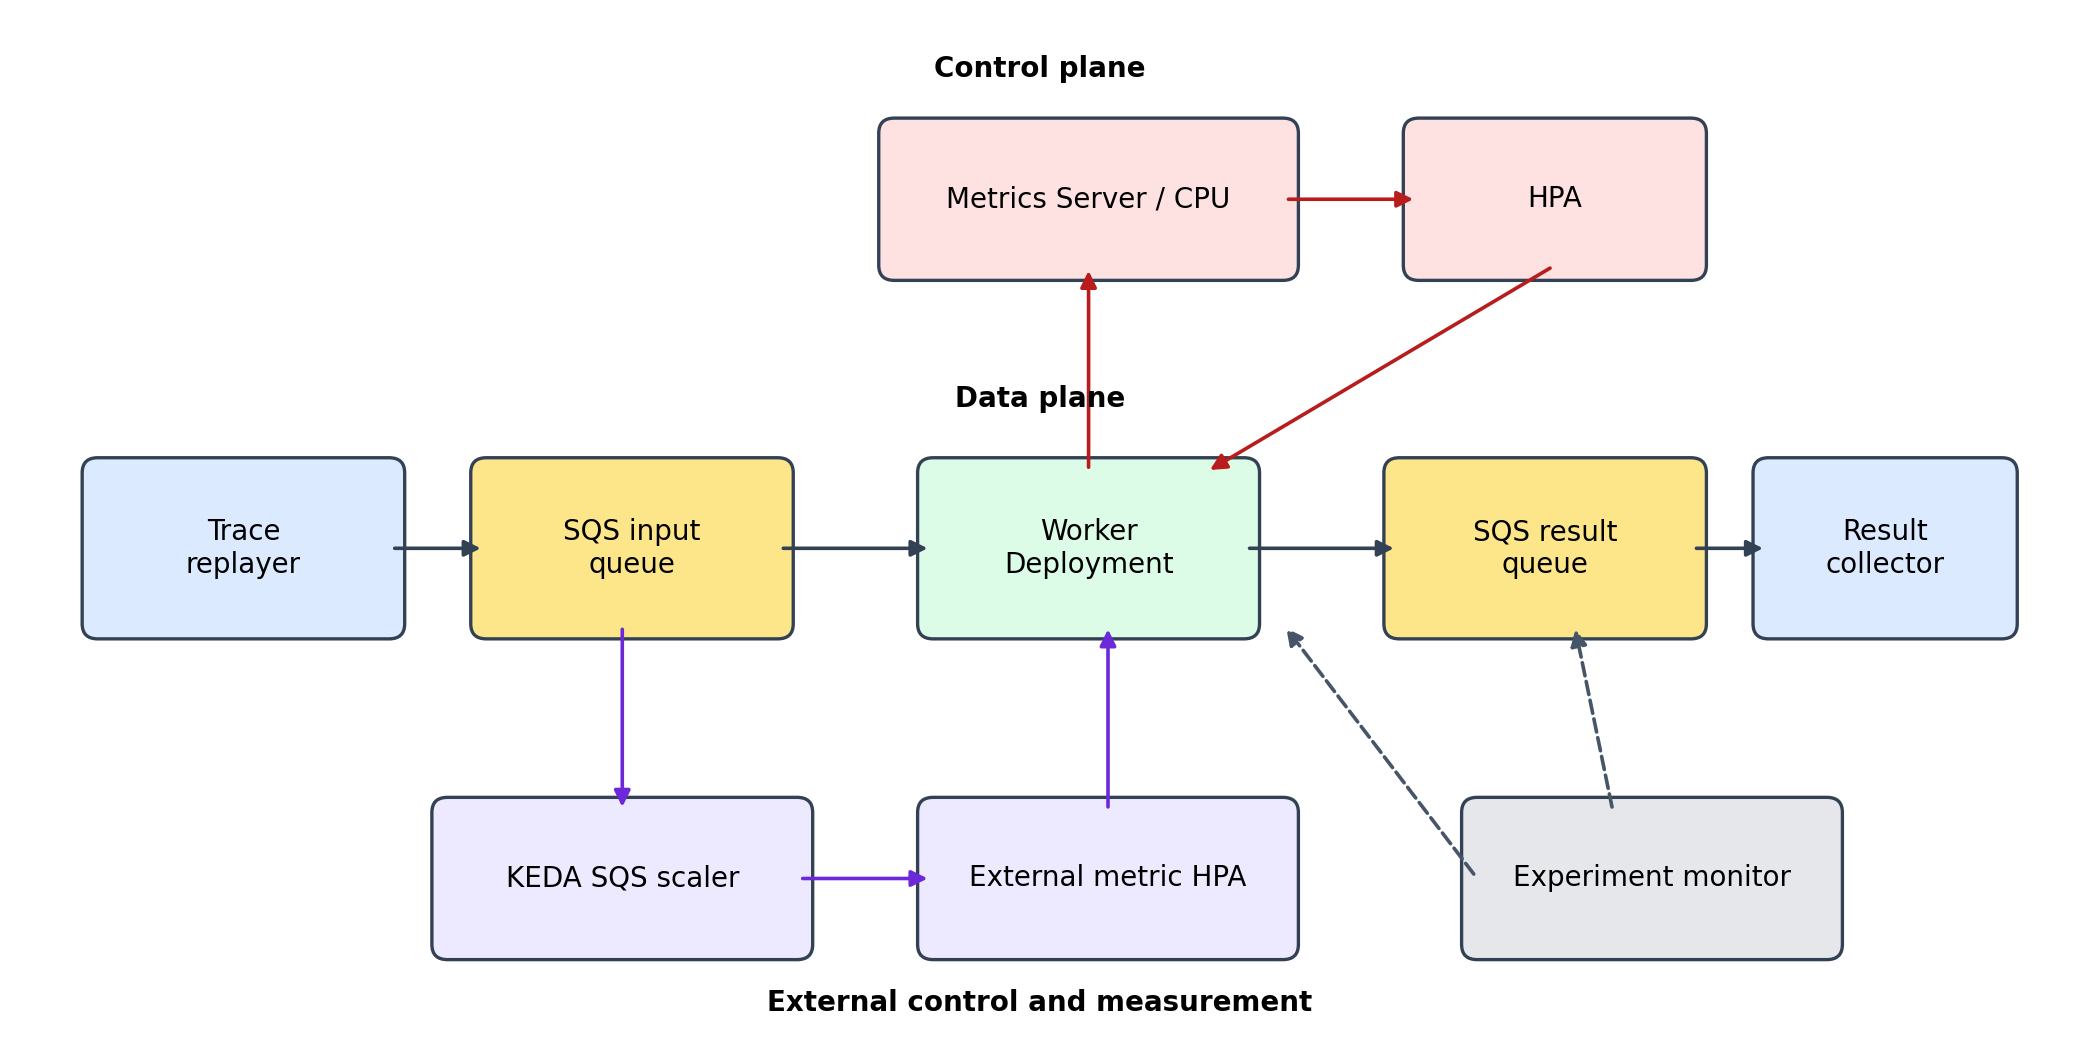
\includegraphics[width=0.93\textwidth]
    {../results/analysis/architecture.png}
  \caption{Experimental architecture. Gray arrows carry messages, red arrows
  show the CPU/HPA path, purple arrows show the SQS/KEDA path, and dashed arrows
  represent independent observation. Only one autoscaling path is active in a
  measured run.}
  \label{fig:architecture}
\end{figure*}

\subsection{Controlled Environment}

Table~\ref{tab:config} summarizes the frozen configuration. Both policies share
one Deployment and differ only in the active autoscaler. KEDA and the worker use
separate IAM roles for service accounts. This follows least privilege and avoids
placing long-lived AWS credentials in Pods \cite{AWSEKSIRSA}.

\begin{table}[t]
  \caption{Frozen Experimental Configuration}
  \label{tab:config}
  \centering
  \begin{tabular}{ll}
    \toprule
    Component & Configuration \\
    \midrule
    Region & \code{us-east-1} \\
    EKS nodes & one \code{c7i-flex.large} \\
    Node scaling & disabled, one node fixed \\
    Worker replicas & minimum 1, maximum 4 \\
    Worker CPU & request 200m, limit 400m \\
    Worker memory & request 96 MiB, limit 192 MiB \\
    HPA signal & CPU, target 60\% of request \\
    KEDA signal & visible plus in-flight SQS messages \\
    KEDA target & 5 messages per Pod \\
    Polling interval & 15 s \\
    Scale-down stabilization & 60 s \\
    Input visibility timeout & 120 s \\
    Trace duration & 180 s \\
    \bottomrule
  \end{tabular}
\end{table}

The cluster has public worker networking and no NAT Gateway. It creates no load
balancer, database, dashboard stack, or node autoscaler. Four workers can consume
at most 1.6 vCPU by cgroup limit, leaving nominal CPU capacity for Kubernetes,
KEDA, and Metrics Server on the 2-vCPU node.

Identical replica limits do not imply equivalent target aggressiveness. Mean
offered CPU demand is approximately $1.6\times0.2=0.32$ CPU. HPA targets 60\%
of a 0.20-CPU request, or 0.12 CPU per replica. Ignoring overhead and sampling,
the mean-load target therefore corresponds to
$\lceil0.32/0.12\rceil=3$ replicas. The 0.40-CPU limit bounds execution but is
not the denominator of HPA utilization. KEDA instead tolerates approximately
five visible-plus-in-flight messages per desired Pod. The experiment compares
these frozen policy configurations; it does not claim that their targets encode
the same latency or capacity objective.

\subsection{Workload Construction}

The common mean arrival rate is 1.6 messages/s. CPU service demand is exponential
with mean 0.2 CPU-s and is clipped to the interval from 0.005 to 1 CPU-s. At a
0.4-CPU Pod limit, one continuously busy replica has an approximate capacity of
2 messages/s before overhead. Thus, the mean load is below one-replica capacity,
while bursts can exceed it.

MMPP rates are 0.4 and 4 messages/s. Transition rates are 0.05/s from low to high
and 0.10/s from high to low. Therefore $\pi_H=1/3$ and the stationary mean is
1.6 messages/s. The chain starts in its stationary distribution. Because a
180-second realization can differ greatly from its stationary mean,
deterministic rejection sampling accepts an MMPP trace only when its count is
within 10\% of the expected count. The base seed, accepted arrival seed,
attempt, empirical rate, offsets, and demands are retained. This rule uses only
offered-load counts and no autoscaling outcome.

Short-window counts verify that equal means did not erase burstiness. Across
nine traces, median maximum arrivals in 1-, 5-, 15-, and 30-second windows were
7, 17, 39, and 63 for Poisson, versus 11, 30, 68, and 103 for MMPP. The median
inter-arrival coefficient of variation was 0.991 and 1.938. MMPP generated a
median 85.1\% of arrivals in the high state. This is close to the theoretical
arrival-weighted fraction

\begin{equation}
  P(H\mid\mathrm{arrival})=
  \frac{\pi_H\lambda_H}{\bar{\lambda}}=\frac{(1/3)4}{1.6}=0.833.
\end{equation}

Figure~\ref{fig:traces} illustrates how cumulative arrivals cluster even when
the final counts are comparable.

\begin{figure}[t]
  \centering
  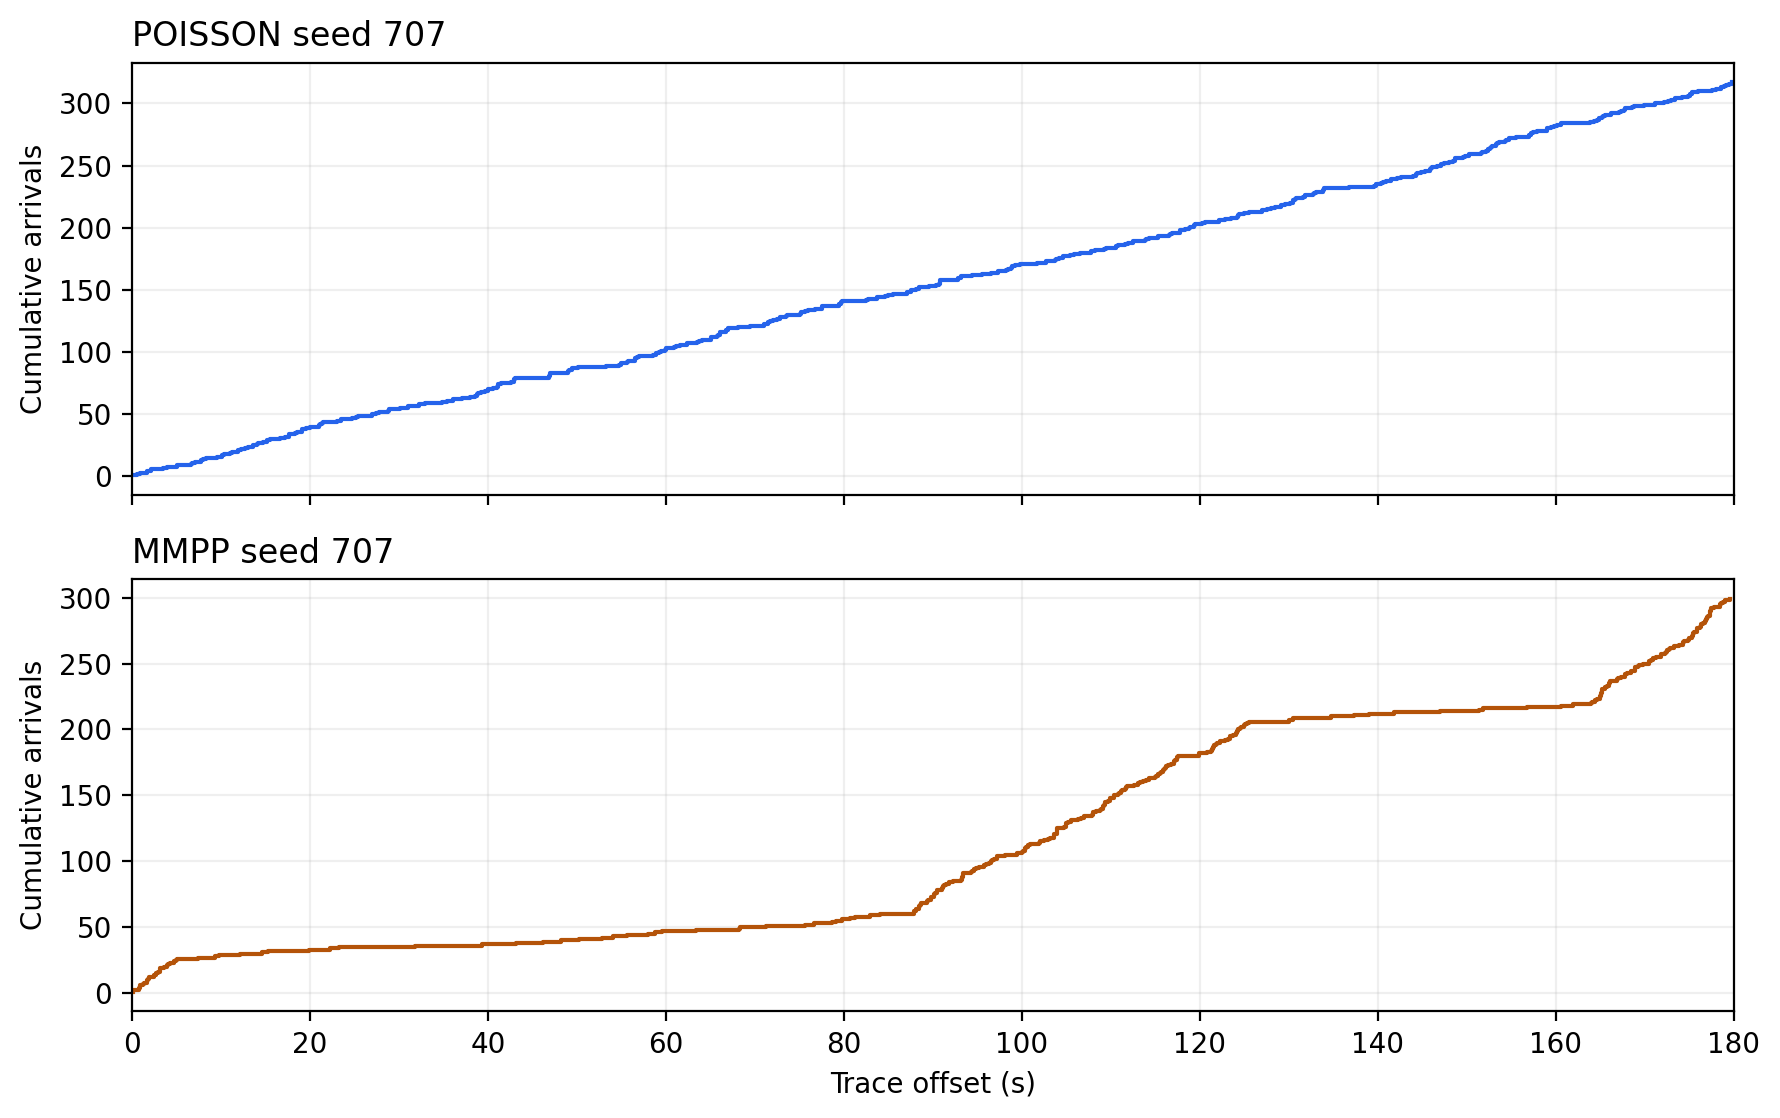
\includegraphics[width=\columnwidth]
    {../results/analysis/trace_comparison.png}
  \caption{Cumulative arrivals for representative seed 707. Changes in MMPP
  slope expose alternating low- and high-rate periods.}
  \label{fig:traces}
\end{figure}

\subsection{Run Procedure}

Before each run, the runner verifies that input and result queues are empty for
three consecutive observations, exactly one worker is ready, the expected
autoscaler is the only active policy, and its status is healthy. The system is
idle for at least 30 seconds before the first arrival. The producer follows
absolute monotonic deadlines and dispatches sends through a bounded thread pool,
preventing one SQS network round trip from delaying later arrivals. It records
scheduling lag when each sender starts its API call.

A collector long-polls the result queue while a monitor samples the Deployment,
Pods, nodes, and both SQS queues every five seconds. Collection continues through
a 15-second quiet window after all unique results arrive, which captures late
duplicates. Configuration snapshots taken before and after the run detect
changes to the Deployment or autoscaler specification.

Table~\ref{tab:timeline} makes the measurement windows explicit. Producer
deadlines use a local monotonic clock, but accepted arrival time comes from the
SQS service response. Worker receipt and completion use the EKS node clock.
Cross-clock subtraction is checked for impossible negative values. The monitor
records desired, ready, available, and pending replicas; node readiness;
restarts; and approximate queue counts independently of message processing.

\begin{table}[t]
  \caption{Measured Run Timeline}
  \label{tab:timeline}
  \centering
  \begin{tabular}{rl}
    \toprule
    Step & Gate or observation \\
    \midrule
    1 & Remove previous policy and reset Deployment \\
    2 & Observe both queues empty three times \\
    3 & Apply one policy and await healthy status \\
    4 & Hold one ready, pre-pulled worker for 30 s \\
    5 & Replay 180-s trace on absolute deadlines \\
    6 & Collect results and sample state every 5 s \\
    7 & Mark last accepted input and last completion \\
    8 & Observe 15-s quiet window for duplicates \\
    9 & Observe scale-down and write final summary \\
    \bottomrule
  \end{tabular}
\end{table}

A run is invalid if producer lag p95 exceeds 250 ms, monitoring has a gap longer
than 15 seconds, a node becomes NotReady, a worker restarts, a Pod is persistently
unschedulable, configuration changes, clock sanity checks fail, or any expected
unique result is missing. Immediate post-run SQS counters are diagnostic because
they are approximate. Failure to obtain a clean three-observation reset before
the next run, a late result, or an unexpected experiment identifier is invalid.
One automatic retry uses the same trace after both queues are purged and the SQS
purge interval has elapsed.

\subsection{Statistical Analysis}

For metric $Y$, each seed and workload yields the paired ratio

\begin{equation}
  R_i=\frac{Y_{i,\mathrm{KEDA}}}{Y_{i,\mathrm{HPA}}}.
\end{equation}

The analysis reports all paired points, the median ratio, and the geometric mean
ratio. A nonparametric paired bootstrap resamples complete ratios with replacement
and uses the 2.5th and 97.5th percentiles for a 95\% interval
\cite{Efron1993Bootstrap}. It also separates runs by treatment order as a
sensitivity analysis. This avoids pseudoreplication from hundreds of correlated
messages within one controller run.

The bootstrap uses 10,000 resamples and a fixed pseudorandom seed of 5120. The
interval is the percentile interval, not bias-corrected and accelerated. Per-run
percentiles use NumPy's default linear interpolation. With 260--327 messages per
run, p95 depends on roughly 13--16 upper-tail observations, another reason to
avoid treating message-level values as independent evidence. The two primary
endpoints were prespecified; no multiplicity-adjusted claims are made for
secondary outcomes.

For the common seeds completed in both workload strata, a descriptive
interaction is

\begin{equation}
  I_i=\frac{R_{i,\mathrm{MMPP}}}{R_{i,\mathrm{Poisson}}}.
\end{equation}

Values above one indicate that the KEDA/HPA ratio increased under MMPP. Because
order and campaign time are not independently balanced in the realized
extension, this quantity supports mechanism discussion rather than a causal
workload-interaction claim.

Queueing relations provide consistency checks rather than a stationary model of
the experiment. For $c$ replicas with service rate $\mu$, the reference
utilization is $\rho=\lambda/(c\mu)$. Little's Law, $L=\lambda W$, is interpreted
cautiously because MMPP arrivals, changing capacity, and finite traces make the
system transient.

\section{Implementation and Reproducibility}

The worker is a non-root Python container. It long-polls one SQS message, validates
the protocol, consumes the requested CPU time, sends a structured result, and
then deletes the input. The result contains SQS acceptance time, worker receipt
and completion times, Pod and node names, receive count, service demand, and a
work digest. CPU time is measured with \code{time.process_time()}, so cgroup
throttling increases wall time without reducing requested CPU work.

Each Pod processes at most one message at a time. It uses 10-second SQS long
polling, requests one message, and sets a 120-second visibility timeout. The
result is sent before input deletion, preserving SQS's at-least-once semantics;
the experiment identifier and job identifier allow the collector to distinguish
duplicates from expected results. The boto3 client uses standard retry mode with
up to eight attempts. These details affect queue residence and are held constant
across policies.

AWS resources are defined by CloudFormation and \code{eksctl}. CloudFormation
creates two SQS queues, one immutable ECR repository, and separate managed
policies for the worker and KEDA. The cluster uses one managed node group,
public networking, and no NAT Gateway. The image tag includes a hash of the
complete worker build context, and the resolved image URI is retained in each
run summary.

The measured environment used EKS Kubernetes 1.34.10 and KEDA 2.17.2. Metrics
Server was installed as the managed EKS add-on. Worker resources, health probes,
autoscaler manifests, queue URLs, image tag, and resolved worker image are
captured by the deployment pipeline or run summary. The image was pre-pulled
before measured execution so treatment order did not determine whether the node
had to download it.

Creation scripts require \code{ALLOW_AWS_CHARGES=YES}. Cleanup independently
requires \code{ALLOW_AWS_DELETE=YES}, verifies the target account and region,
deletes IRSA roles before the cluster and foundation stack, and audits EKS,
EC2, EBS, NAT, Elastic IP, load balancer, CloudFormation, SQS, ECR, IAM, and log
resources. The design keeps the expected session cost below USD 2 and the
explicit ceiling at USD 20.

The repository includes unit tests for deterministic traces, workload bounds,
message validation, temporal integration, manifest parsing, paired analysis,
and the sequential stopping decision. The worker image, CloudFormation template,
and \code{eksctl} configuration are also validated before cloud creation.

\subsection{Retained Artifacts and Auditability}

Each completed attempt directory contains producer events, accepted result
messages, Kubernetes and SQS monitor samples, duplicate records, and a
machine-readable summary. Immutable traces are retained separately by pattern
and seed. Analysis discovers summaries recursively but accepts only records
marked as main-campaign and valid. It then joins policies by workload and seed,
so an interrupted or unpaired attempt cannot silently enter a paired estimate.

The analysis writes both tabular CSV outputs and publication figures. Its
campaign-status record distinguishes planned runs, valid completed runs,
complete pairs, and cells not executed. Reproduction therefore does not depend
on console logs or values transcribed from this paper. The final lifecycle audit
uses service-specific list operations instead of assuming that successful stack
deletion implies complete cleanup.

\section{Results}

\subsection{Campaign Integrity}

The measured campaign produced 35 valid main runs: 18 Poisson runs and 17 MMPP
runs. These runs processed between 271 and 327 Poisson messages and between 260
and 310 MMPP messages. All expected messages produced exactly one accepted
result. No run had a missing result, worker restart, NotReady node, persistent
unschedulable Pod, or configuration change. Median producer lag p95 was 1.93 ms
for Poisson and 2.77 ms for MMPP, far below the 250-ms validity threshold. The
largest monitoring gap was 8.98 s, also below its 15-s threshold.

\begin{table}[t]
  \caption{Realized Main Campaign}
  \label{tab:campaign}
  \centering
  \begin{tabular}{lr}
    \toprule
    Campaign item & Count \\
    \midrule
    Planned treatment cells & 40 \\
    Valid completed cells & 35 \\
    Complete Poisson pairs & 9 \\
    Complete MMPP pairs & 8 \\
    Valid but unpaired cells & 1 \\
    Missing or duplicate accepted results & 0 \\
    Worker restarts or NotReady nodes & 0 \\
    Remaining AWS project resources & 0 \\
    \bottomrule
  \end{tabular}
\end{table}

The first five pairs failed the predefined interval-precision criterion, so the
campaign entered its five-seed extension. Extended cloud runtime and repeated
short-lived login interruptions led to termination after nine complete Poisson
pairs and eight complete MMPP pairs. One additional HPA/MMPP run had no KEDA
counterpart and was excluded from all paired estimates. No value was imputed.
Consequently, the results retain more replication than the initial stage but do
not claim completion of the planned ten-pair maximum. The AWS cleanup audit
subsequently found no remaining project resource.

Table~\ref{tab:traces} characterizes the nine generated traces of each pattern.
The mean empirical rates were close, but median inter-arrival coefficient of
variation was approximately twice as large for MMPP. Most MMPP messages arrived
in the high state even though that state occupies one third of stationary time,
as expected because arrivals are sampled more frequently while its rate is high.

\begin{table}[t]
  \caption{Retained Workload Trace Characteristics}
  \label{tab:traces}
  \centering
  \begin{tabular}{lrrrr}
    \toprule
    Pattern & Traces & Jobs range & Mean rate & Median IAT CV \\
    \midrule
    Poisson & 9 & 271--327 & 1.627 & 0.991 \\
    MMPP & 9 & 260--310 & 1.609 & 1.938 \\
    \bottomrule
  \end{tabular}
\end{table}

\subsection{Primary Outcomes}

Table~\ref{tab:primary} reports KEDA/HPA ratios. A ratio above one indicates a
larger outcome under KEDA. For Poisson traces, the geometric-mean p95 latency
ratio was 2.03 (95\% bootstrap interval 1.44--2.81). For MMPP traces, it was
2.66 (1.56--4.73). HPA therefore had lower aggregate p95 latency under both
arrival patterns in this configuration. These paired bootstrap uncertainty
intervals exclude one, but the small realized sample and MMPP order confounding
preclude a broad confirmatory claim.

\begin{table}[t]
  \caption{Paired Primary Outcomes, KEDA/HPA Ratio}
  \label{tab:primary}
  \centering
  \begin{tabular}{llrrr}
    \toprule
    Pattern & Outcome & $n$ & Geo. mean & 95\% CI \\
    \midrule
    Poisson & Latency p95 & 9 & 2.033 & [1.436, 2.810] \\
    Poisson & Pod-seconds & 9 & 0.522 & [0.486, 0.560] \\
    MMPP & Latency p95 & 8 & 2.659 & [1.558, 4.728] \\
    MMPP & Pod-seconds & 8 & 0.701 & [0.581, 0.823] \\
    \bottomrule
  \end{tabular}
\end{table}

The corresponding ready pod-seconds ratios were 0.522 (0.486--0.560) for
Poisson and 0.701 (0.581--0.823) for MMPP. KEDA thus had 47.8\% and 29.9\%
less ready-capacity exposure, respectively. The Poisson pod-seconds interval met the
predefined plus-or-minus 10\% precision criterion. The other three intervals
did not. Figures~\ref{fig:latency} and~\ref{fig:pods} expose every paired point
rather than only the aggregate estimates.

Direction counts reinforce the trade-off without treating messages as
replicates. KEDA used fewer ready pod-seconds in all 17 pairs. HPA had lower p95
latency in 16 of 17 pairs. The only exception was Poisson seed 101, for which the
latency ratio was 0.757. Every MMPP ratio exceeded one, although seed 505 was
nearly equal at 1.013. Thus, the aggregate directions were not produced by one
isolated outlier, even though effect magnitude varied considerably.

\begin{figure}[t]
  \centering
  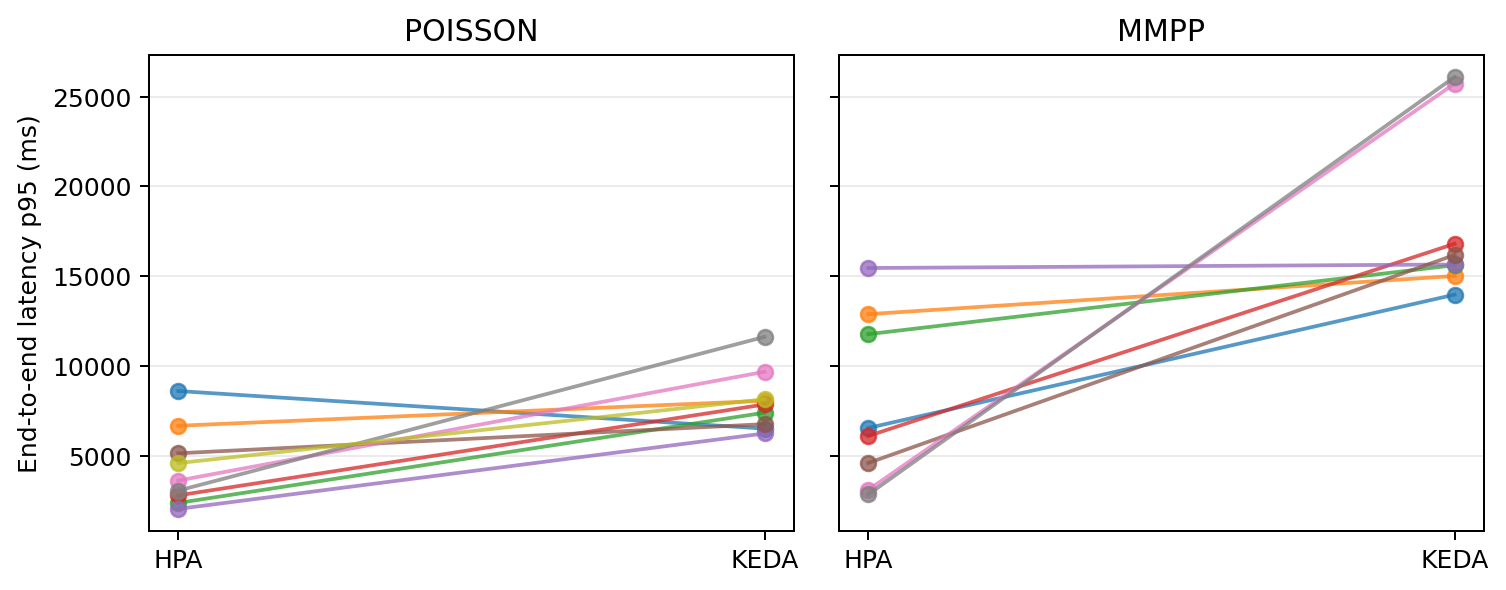
\includegraphics[width=\columnwidth]
    {../results/analysis/paired_latency_ms_p95.png}
  \caption{Per-trace p95 latency under HPA and KEDA. The dashed diagonal marks
  equal outcomes; points above it favor HPA.}
  \label{fig:latency}
\end{figure}

\begin{figure}[t]
  \centering
  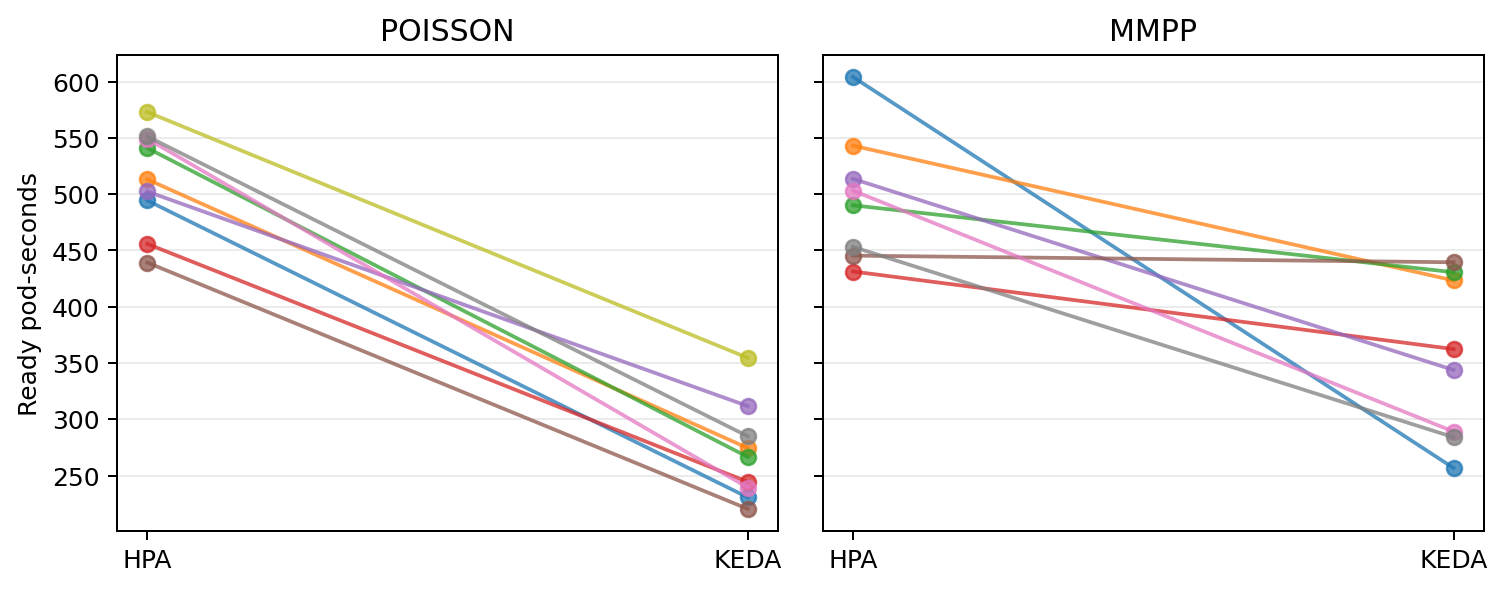
\includegraphics[width=\columnwidth]
    {../results/analysis/paired_ready_pod_seconds.png}
  \caption{Per-trace ready pod-seconds. Points below the equal-outcome diagonal
  indicate lower ready-capacity exposure under KEDA.}
  \label{fig:pods}
\end{figure}

\subsection{Scaling and Backlog Behavior}

Paired-only medians explain the primary trade-off without mixing the unpaired
HPA/MMPP seed 909 into one policy. Under Poisson traffic, median p95 latency was
3.605 s for HPA and 7.845 s for KEDA, while median ready pod-seconds were 513.1
and 266.5. Median peak replica count was four for HPA and two for KEDA. Median
maximum backlog was nine messages under HPA and 15 under KEDA. Median time from
workload start until an additional Pod became ready was 36.8 s for HPA and 81.5
s for KEDA.

For the eight paired MMPP seeds, median p95 latency was 6.312 s for HPA and
15.907 s for KEDA, and median ready pod-seconds were 496.6 and 353.1. Both
policies had a median peak of four replicas, but median maximum backlog was 16
for HPA and 39 for KEDA. Median workload-start-to-ready time was 46.8 and 54.3
s. This metric includes trace timing, sensing, reconciliation, scheduling, and
readiness; it is not a direct measurement of controller polling delay.

Table~\ref{tab:secondary} reports exploratory mechanism ratios. Queue-wait p95
was 2.82 times larger with KEDA for Poisson and 3.01 times larger for MMPP.
Integrated backlog ratios were 2.13 and 2.58. Queue residence therefore explains
much of the end-to-end latency difference. KEDA reached lower peak capacity,
especially under Poisson, while observed scale-out to a ready Pod occurred
later on average.

\begin{table}[t]
  \caption{Exploratory Secondary KEDA/HPA Ratios}
  \label{tab:secondary}
  \centering
  \begin{tabular}{lrr}
    \toprule
    Outcome & Poisson & MMPP \\
    \midrule
    Mean end-to-end latency & 2.124 & 2.515 \\
    Queue-wait p95 & 2.816 & 3.006 \\
    Integrated backlog & 2.134 & 2.580 \\
    Maximum sampled backlog & 1.823 & 2.134 \\
    Workload-start-to-ready & 1.675 & 1.370 \\
    Peak ready replicas & 0.599 & 0.885 \\
    \bottomrule
  \end{tabular}
\end{table}

The direction was again consistent. Integrated backlog favored HPA in all nine
Poisson pairs and seven of eight MMPP pairs. Queue-wait p95 favored HPA in eight
of nine Poisson and seven of eight MMPP pairs. KEDA reached a lower peak replica
count in all nine Poisson pairs; under MMPP it was lower in two and tied in six.
These secondary comparisons were not multiplicity-adjusted and should be read
as mechanism evidence rather than additional hypothesis tests.

Figure~\ref{fig:backlog} shows that MMPP outcomes were heterogeneous. KEDA
controlled maximum backlog on some traces but accumulated much larger peaks on
others. This variation is consistent with sensitivity to the timing and length
of high-state intervals, which equal message counts alone do not control.

\begin{figure}[t]
  \centering
  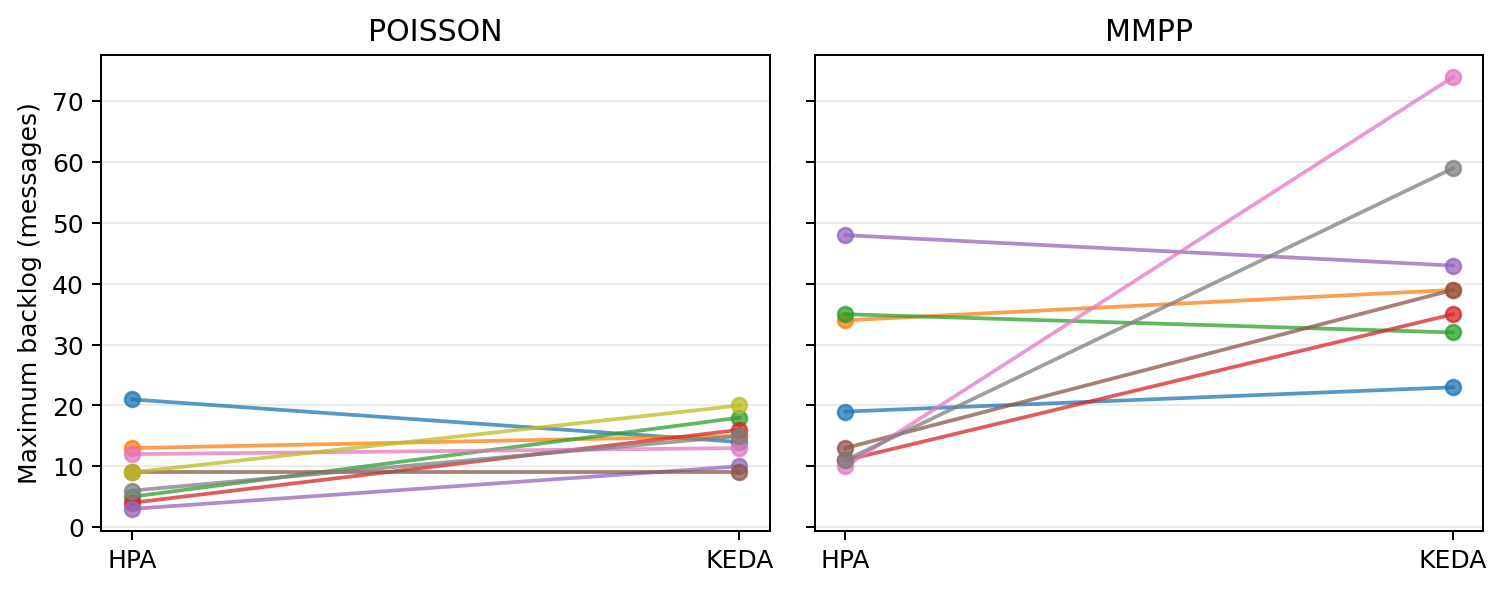
\includegraphics[width=\columnwidth]
    {../results/analysis/paired_max_backlog.png}
  \caption{Per-trace maximum observed backlog. Lower points indicate stronger
  backlog containment during the finite workload.}
  \label{fig:backlog}
\end{figure}

\subsection{Observed Control Timing and Replica Occupancy}

Five-second monitor samples permit a coarse decomposition between a change in
desired count and a subsequently observed ready Pod. Table~\ref{tab:timing}
reports medians aligned to the first sample after workload start. Under Poisson,
HPA first requested more than one replica after 31.6 s, while KEDA did so after
74.9 s. Desired-to-ready time was actually shorter for KEDA, indicating that the
large total difference primarily preceded its scale request. Under MMPP, KEDA
requested capacity 6.6 s later and had a longer observed desired-to-ready phase.

\begin{table}[t]
  \caption{Median Sampled Scaling Times from Workload Start}
  \label{tab:timing}
  \centering
  \begin{tabular}{llrrr}
    \toprule
    Pattern & Policy & Desired $>1$ & Ready $>1$ & Difference \\
    \midrule
    Poisson & HPA & 31.6 s & 35.1 s & 10.0 s \\
    Poisson & KEDA & 74.9 s & 80.0 s & 5.2 s \\
    MMPP & HPA & 31.7 s & 44.9 s & 6.6 s \\
    MMPP & KEDA & 38.3 s & 52.6 s & 10.4 s \\
    \bottomrule
  \end{tabular}
\end{table}

The difference column is computed within runs before taking the median, so it
need not equal the difference between the preceding median columns. Sampling
interval-censors all three values by roughly five seconds. Moreover, the data do
not expose Metrics Server freshness, KEDA's exact poll instant, or internal HPA
reconciliation separately. The safe conclusion is that KEDA's observed desired
count changed later under Poisson, not that any single internal component caused
the full delay.

\begin{figure}[t]
  \centering
  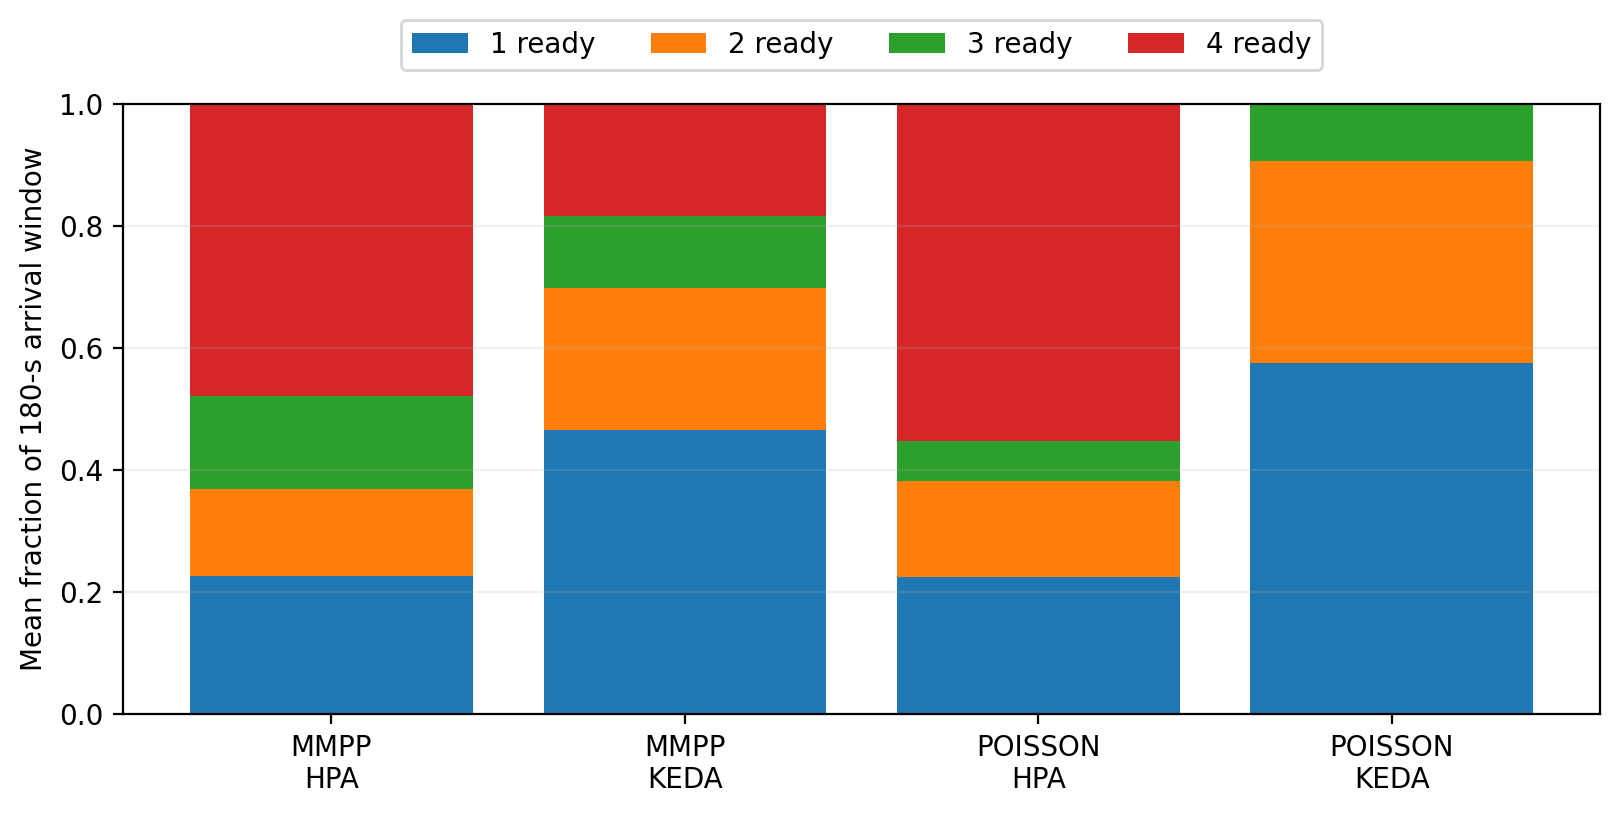
\includegraphics[width=\columnwidth]
    {../results/analysis/replica_occupancy.png}
  \caption{Mean fraction of the 180-second arrival window observed at each ready
  replica count. The distribution explains differences in ready pod-seconds.}
  \label{fig:occupancy}
\end{figure}

Figure~\ref{fig:occupancy} directly links replica occupancy to pod-seconds.
Poisson KEDA spent about 57.6\% of the arrival window at one ready Pod and did not
reach four in the mean occupancy profile. Poisson HPA spent about 55.3\% at four.
MMPP drove both policies higher, but HPA still spent a larger share at four
ready replicas. These observations explain why KEDA reduced ready-capacity
exposure while allowing a larger queue.

Figure~\ref{fig:timeline} presents one high-contrast pair rather than an
aggregate. For MMPP seed 707, the same frozen trace produced an HPA p95 of 3.09
s and a KEDA p95 of 25.72 s. KEDA's sampled backlog peaked at 74 messages versus
10 for HPA. The timeline shows repeated bursts, delayed desired-count changes,
and the gap between desired and ready capacity. It is illustrative; the paired
estimates continue to use all complete seeds.

\begin{figure}[t]
  \centering
  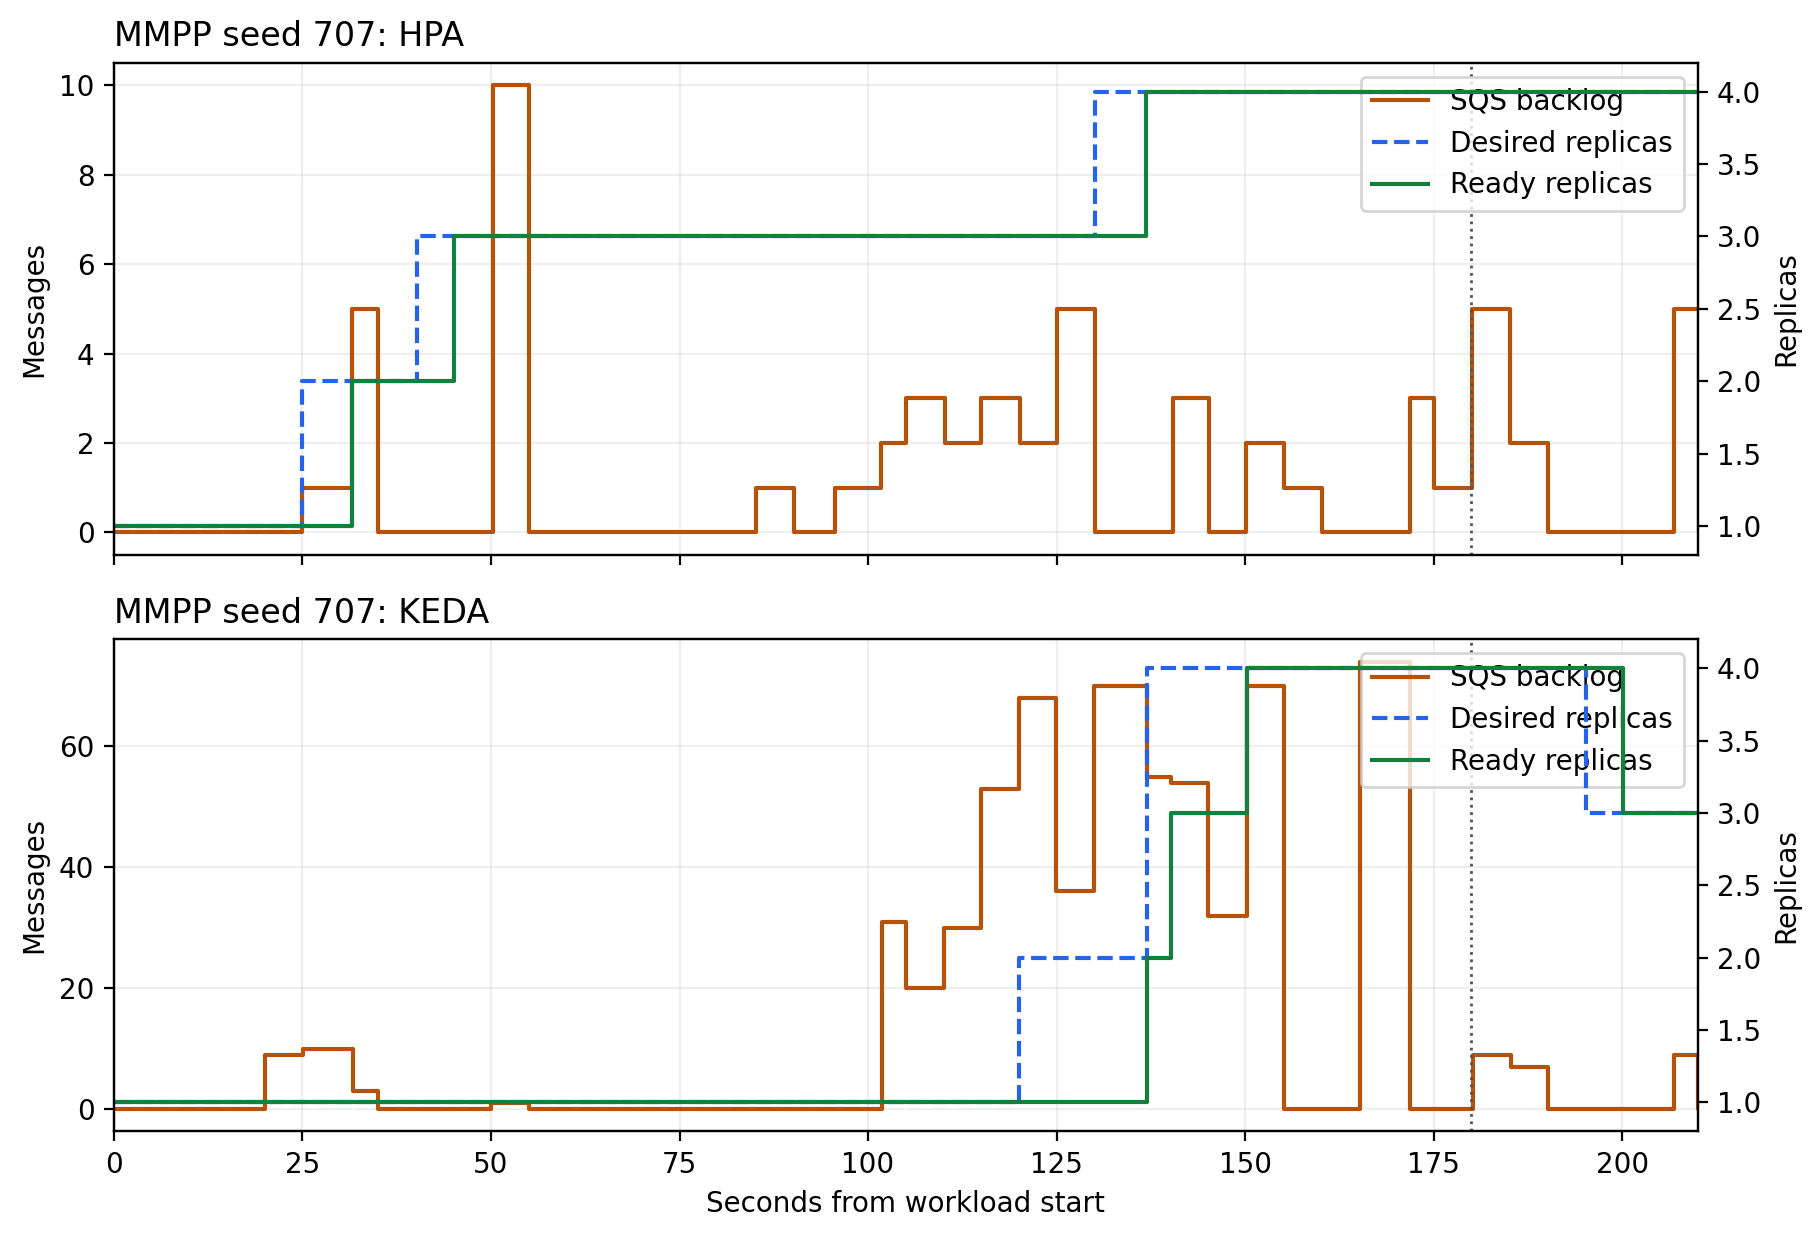
\includegraphics[width=\columnwidth]
    {../results/analysis/mmpp_seed707_timeline.png}
  \caption{Backlog, desired replicas, and ready replicas for the MMPP seed 707
  pair. The dotted vertical line marks the end of the 180-second arrival trace.}
  \label{fig:timeline}
\end{figure}

\subsection{Order and Workload Sensitivity}

Treatment-order sensitivity was stable for ready pod-seconds but not for
latency. For Poisson, geometric-mean pod-second ratios were 0.524 when HPA ran
first and 0.519 when KEDA ran first. For MMPP they were 0.708 and 0.696.
Geometric-mean latency ratios were 2.39 versus 1.66 for Poisson and 6.47 versus
1.56 for MMPP. Figure~\ref{fig:order} makes the seed progression visible.

\begin{figure}[t]
  \centering
  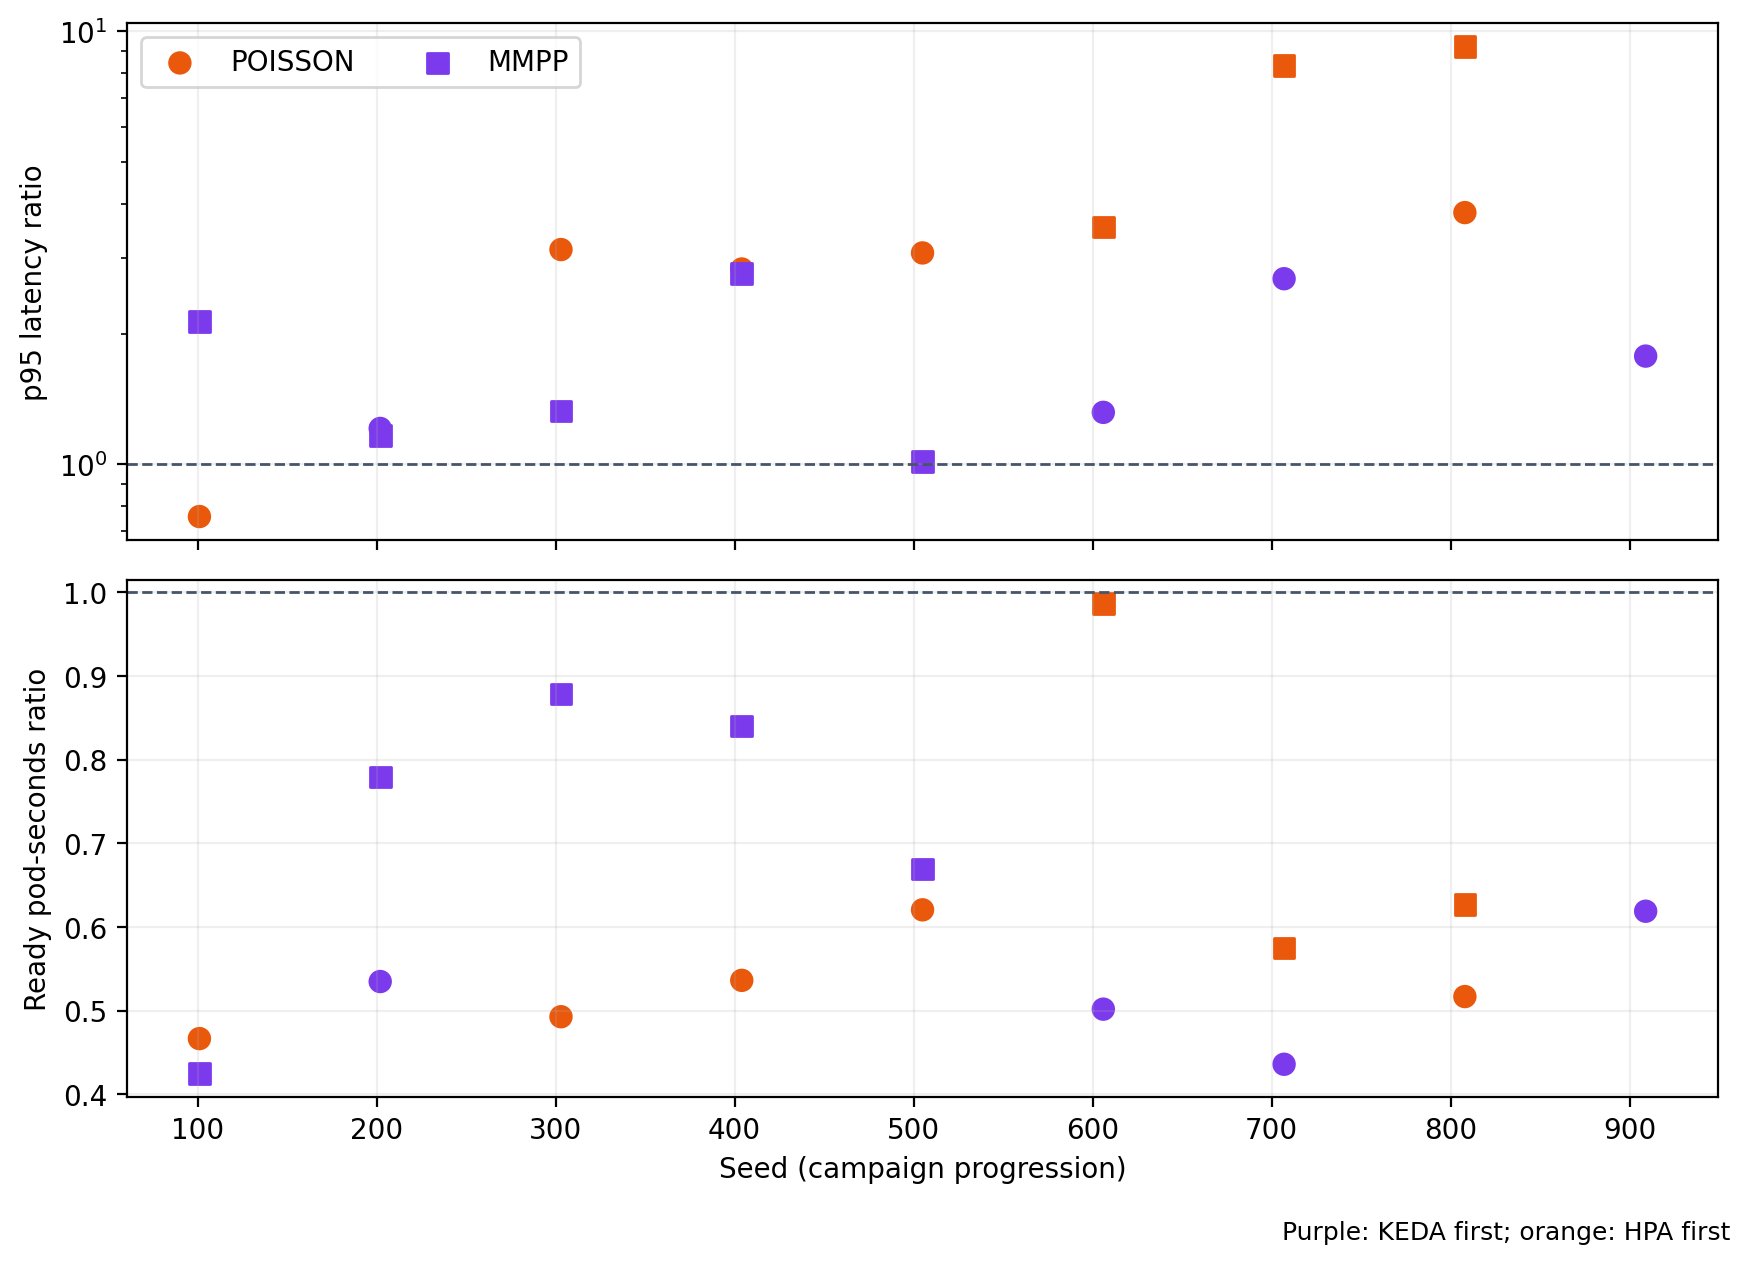
\includegraphics[width=\columnwidth]
    {../results/analysis/order_sensitivity.png}
  \caption{Primary KEDA/HPA ratios by seed and treatment order. Purple denotes
  KEDA first and orange HPA first; seed also tracks campaign progression.}
  \label{fig:order}
\end{figure}

The MMPP schedule is critically limited: KEDA ran first for seeds 101--505,
whereas HPA ran first for all complete extension seeds 606--808. The three late
latency ratios were 3.53, 8.33, and 9.21. Treatment order, seed block, and
campaign time are therefore completely confounded in that portion of the MMPP
data. The overall MMPP latency ratio remains an accurate description of the
executed pairs, but its magnitude cannot be assigned solely to autoscaler choice.

Across the eight seeds complete in both workload strata, the geometric-mean
MMPP/Poisson ratio-of-ratios was 1.286 for p95 latency and 1.373 for ready
pod-seconds. The respective uncertainty intervals were 0.709--2.211 and
1.158--1.618. Descriptively, burstiness reduced KEDA's relative ready-capacity
advantage and may have amplified its latency disadvantage, but latency
heterogeneity and the order confounding prevent a causal interaction claim.

\section{Discussion}

\subsection{Target Calibration Dominated Signal Proximity}

The experiment does not support the intuitive claim that observing the queue
necessarily improves tail latency. KEDA observed a signal closer to external
demand, but the selected target of five messages per Pod preserved fewer active
Pods during the mostly sub-capacity mean load. HPA's 60\% CPU target instead
kept or requested more capacity once work reached a consumer. In this setting,
that aggressive capacity response outweighed the informational advantage of the
queue signal.

The nominal HPA calculation in Section III-C helps explain why. The 60\% target
is relative to the 200m request, not the 400m limit. Its 120m target utilization
per replica is low compared with the 320m mean offered CPU demand, so three
replicas are an idealized equilibrium before overhead. KEDA can remain at one
replica until its sampled backlog justifies another. The observed Poisson
desired-count times support this mechanism: KEDA's larger delay occurred before
the Deployment requested a second Pod, not primarily while that Pod became
ready.

During an MMPP high state, the arrival rate rises to 4 messages/s. With an
idealized one-Pod service rate near 2 messages/s, at least two continuously busy
Pods are needed merely to match new arrivals. Work accumulates while sensing and
startup occur, and additional capacity must both serve new arrivals and drain
the queue. This transient explanation is more appropriate than a stationary
queueing model because capacity and arrival state both change during a
180-second trace.

\subsection{A Ready-Capacity and Latency Trade-off}

The trade-off was directionally consistent: all 17 ready pod-second contrasts
favored KEDA, while 16 of 17 p95 latency contrasts favored HPA. This does not
mean KEDA reduced the actual AWS bill. The EC2 node and EKS control plane were
allocated for both treatments. Ready pod-seconds instead quantify how much
consumer capacity the policy exposed within that fixed infrastructure. They can
matter on clusters where freed requests permit other workloads or node
consolidation, but neither consequence was measured here.

These findings apply to policy configurations, not controller brands in the
abstract. A smaller KEDA backlog target, shorter polling interval, higher
minimum replica count, or predictive activation could spend more pod-seconds to
reduce waiting. Conversely, a higher HPA CPU target or longer stabilization
could save capacity at a latency cost. The practical implication is that a
queue-aware metric still requires a target aligned with a service-level
objective; metric proximity alone does not guarantee responsiveness.

An operator choosing between these configurations should therefore start from
an SLO and a capacity budget. The measured KEDA setup may suit throughput-first
workloads that tolerate queueing and value lower ready-capacity exposure. The
measured HPA setup better protected latency by maintaining more replicas. A
stronger policy comparison would tune HPA CPU targets and KEDA queue targets to
equal latency or equal pod-second budgets, then compare the resulting Pareto
front rather than assuming that equal replica bounds establish fairness.

\subsection{Burstiness and Mechanism Uncertainty}

Descriptively, MMPP reduced KEDA's relative pod-second advantage from about 48\%
to 30\%, while its latency ratio increased from 2.03 to 2.66. This pattern is
plausible because high states pushed both policies toward the four-replica
ceiling. It is not a clean causal workload effect: the ratio-of-ratios latency
interval includes one, and late MMPP seeds are confounded with treatment order
and campaign time.

The monitor establishes desired and ready replica timing, but cannot isolate
every delay. Metrics Server freshness, KEDA polling, SQS counter approximation,
HPA reconciliation, scheduler latency, and container readiness all remain
combined or partially observed. Claims about those components are mechanisms
consistent with the data, not direct component-level measurements. Future work
should retain autoscaler events, HPA conditions, CPU samples, external metric
values, scheduling timestamps, and image-start timestamps.

The results also illustrate why per-message significance tests would be
misleading. Hundreds of messages in one trace share the same burst history,
controller state, node, and Pods. Pairing at trace level yields only eight or
nine independent contrasts per workload and appropriately exposes uncertainty
and temporal sensitivity.

\section{Threats to Validity}

\subsection{Internal Validity}

The strongest internal threat is the realized MMPP order schedule. KEDA ran
first for seeds 101--505 and HPA first for complete seeds 606--808. Order, seed
block, and later campaign time cannot be separated. Sequential execution on one
cluster also permits temporal variation in AWS control-plane latency, network
conditions, node state, and background system Pods. Reset gates, pre-pulling,
paired traces, and order reporting reduce but do not eliminate these effects.

The extension stopped with nine Poisson and eight MMPP pairs rather than ten of
each. This non-protocol termination weakens precision and leaves one valid HPA
run unpaired. The analysis excludes that run from every paired estimate and does
not impute missing cells. Transparent exclusion prevents a fabricated pair but
cannot recover the intended balance.

\subsection{Construct Validity}

Ready pod-seconds represent integrated ready replica count, not CPU work,
energy, monetary cost, or useful throughput. A ready but idle Pod contributes
equally to a busy Pod. Likewise, scale-out time begins at workload start, not at
the unobserved instant when a true controller threshold is crossed. The sampled
desired-count decomposition improves interpretation but remains interval
censored.

SQS queue attributes are approximate and sampled every five seconds. Timestamp
subtraction relies on AWS service time and the EKS node clock; negative values
beyond a small tolerance invalidate a run, but small positive clock offsets
cannot be separated from queue wait. Pod-seconds use zero-order-hold integration
between samples and are consequently discretized. Maximum backlog is the largest
sampled approximate value, not the true continuous-time queue maximum.

Immediate post-run queue counters are retained but are not used alone as an
invalidity condition because SQS exposes eventual approximations. Instead, the
next run requires three consecutive empty observations after a bounded wait,
and the collector rejects results carrying another experiment identifier.

\subsection{Statistical Conclusion Validity}

Eight or nine complete pairs provide limited bootstrap support, especially for
wide MMPP effects. Percentile bootstrap intervals inherit the empirical sample's
coarse tails and do not correct bias. Per-run p95 itself is estimated from only
about 13--16 upper-tail messages. The sequential precision check and subsequent
operational termination further complicate nominal interval interpretation.
Individual points, direction counts, and sensitivity analyses make variation
visible but do not create additional independent units.

Only latency p95 and ready pod-seconds were primary. Queue wait, backlog,
replica timing, peak replicas, and interaction ratios are exploratory and
correlated. Their intervals and direction counts receive no multiplicity
correction and should not be interpreted as separate confirmatory tests.

\subsection{External Validity and Reproducibility}

The experiment uses one AWS region, one cluster, one node type, one CPU-bound
worker implementation, standard SQS queues, one replica range, and one set of
controller parameters. Results do not establish universal superiority. I/O-bound,
batched, multithreaded, heterogeneous, or poison-message workloads may behave
differently. The fixed node removes node-autoscaling variation but caps capacity;
persistent unschedulability and node readiness failures were validity gates.

Conditioning MMPP traces on total count improves comparability of offered load
but excludes unusually high- or low-count short realizations. The temporal
clustering remains stochastic and recorded. Longer traces would include more
state transitions and reduce dependence on a few bursts. KEDA was pinned, but
managed EKS and add-on builds may evolve even with the retained Kubernetes
version and manifests. Reproduction therefore requires reporting current cloud
versions in addition to using the archived code and traces.

\section{Conclusion}

For the tested EKS worker and controller settings, CPU-based HPA provided lower
end-to-end p95 latency, whereas SQS-based KEDA had fewer ready pod-seconds.
KEDA/HPA geometric-mean latency ratios were 2.03 under Poisson and 2.66 under
MMPP. Ready pod-seconds ratios were 0.522 and 0.701, equivalent to reductions of
47.8\% and 29.9\% in ready-capacity exposure, not direct monetary cost. KEDA
also had larger median backlogs and later observed ready scale-out in this
configuration, so queue visibility alone did not overcome the combined effects
of target selection and control-path delay.

The result is a configuration-specific trade-off rather than a universal policy
ranking. It demonstrates a reproducible way to compare internal resource
pressure with external queued demand using frozen traces, run-level pairing,
validity gates, retained raw observations, and audited cloud cleanup. Future
work should vary the backlog and CPU targets, add longer traces and independent
clusters, capture controller-internal metrics, and complete a balanced randomized
campaign to separate treatment order from temporal drift. The strongest next
comparison would estimate a latency-capacity Pareto front by tuning both policies
to common SLO or pod-second budgets.

\bibliographystyle{IEEEtran}
\bibliography{references}

\end{document}
